\documentclass[12pt]{article}

% ----- Preamble
\usepackage[utf8]{inputenc} % police encodee en latin1=iso8859-1=Windows Latin 1 %
\usepackage[french]{babel} % police fr %
\usepackage{hyperref} % pour les references %
\usepackage{amsmath} % pour les formules de maths %
\usepackage{amssymb} % pour les symboles maths %
\usepackage{amsthm} % pour la mise en forme des theoremes %
\usepackage{aeguill} % pour les guillemets et accents francais %
\usepackage{listings} % pour les listings de code %
\usepackage{helvet} % police helvetica %
\usepackage{graphicx}
\usepackage{centernot}

% modification des dimensions de la page et de son centrage %
\topmargin -2.0cm
\oddsidemargin 0.2cm
\textwidth 16cm 
\textheight 21cm
\footskip 0.0cm

\title{Traitement d'Image et du Signal - TP3}
\author{Laurent Cetinsoy, Karim Kouki, Aris Tritas }
\date{\today}

\begin{document}
\maketitle

\begin{abstract}
L'objectif de ce TP est de calculer des convolutions, vérifier la validité de filtres linéaires, extraire leur réponse impulsionnelle. Par ailleus nous mettons en pratique la méthode de rotation par distortion de Yarolavsky.
\end{abstract}

\section*{Introduction}
Nous avons donné, lors du TP précédent, l'idée d'algorithme faisant une rotation efficace dans l'espace réel par succession de translations dans le domaine de Fourier. Par souçis de complétude, nous la ré-écrivons ci-suit.

\section*{Rotation d'image}
Pour chaque point $(x, y)$ de l'image originale nous souhaitons utiliser la TFD pour calculer le point $(x', y')$ résultant d'une rotation d'angle  $\theta \in {[0, 2\pi]}$. L'on peut définir la rotation par la matrice \textbf{M} ci-dessous:
$$\begin{pmatrix}
x' \\ y'
\end{pmatrix}=
\begin{pmatrix}
\cos \theta & -\sin \theta \\
\sin \theta & \cos \theta
\end{pmatrix}
\begin{pmatrix}
x \\ y
\end{pmatrix}=\textbf{M}
\begin{pmatrix}
x \\ y
\end{pmatrix}
$$
où \textbf{M} peut être ré-exprimée comme suit (e.g. \cite{paeth86}):
$$M =
\begin{pmatrix}
1 & -\tan \frac{\theta}{2} \\
0 & 1
\end{pmatrix}
\begin{pmatrix}
1 & 0 \\
\sin \theta & 1
\end{pmatrix}
\begin{pmatrix}
1 & -\tan \frac{\theta }{2}\\
0 & 1
\end{pmatrix}
$$
L'idée de \cite{unser95} \cite{larkin97} est d'utiliser trois convolutions linéaires (et donc séparables) qui distordent l'image successivement selon les axes $x$, $y$ et $x$. 
Chacune s'écrit comme une translation dans le domaine de Fourier. La distortion $u_{dx}(x, y) = u(x + ay, y)$ pour l'axe $x$ (où $a$ contrôle l'angle) s'exprime par l'opérateur suivant:
$$ D_x(\xi) = \mathcal{F}\{u_d(x, y)\} = \mathcal{F}\{u(x, y)\} e^{-2 i \pi \xi a y}$$
Le signal réel distordu sur $x$ par la transformée inverse : $ u_{dx}(x, y) = \mathcal{F}^{-1}\{D_x(\xi) \} $ \newline
Si l'on répête cette opération pour $y$ et encore une fois pour $x$ l'on retrouve le signal réel pivoté. Il s'agit bien de trois translations, donc un algorithme efficace qui les effectue peut être donné. A noter que cette méthode induit une perte d'information près des bords, il devient donc nécessaire d'envisager une convolution plus robuste pour parer à cet effet-là.

\section*{Exercices}

Notons le signal d'entrée $e(t)$ et le signal de sortie $s(t)$.


\textbf{Définition} Système linéaire: \newline
Si $e_1(t) \rightarrow s_1(t)$ et $e_2(t) \rightarrow s_2(t)$, alors $\alpha_1 e_1(t) + \alpha_2 e_2(t) \rightarrow \alpha_1 s_1(t) + \alpha_2 s_2(t)$

\textbf{Définition} Système invariant: \newline
Si $e(t) \rightarrow s(t)$ alors $e(t-\tau) \rightarrow s(t-\tau)$, $\tau$ étant une constante de décalalage.

\textbf{Définition} Réponse impulsionnelle: \newline
La sortie d'un système linéaire invariant est égale au produit de convolution de l'entrée par la réponse impulsionnelle $h$. $$e(t) \longrightarrow s(t) = (e \otimes h)(t)$$

\textbf{Définition} Produit de convolution de deux suites $u_n$ et $v_n$: \newline
$$ (u \otimes h)(n) = \sum_{k \in \mathbb{Z}} u_{n-k}h_k $$

\subsection*{Exercice 1}
Pour les questions (1)-(4), l'entrée est la suite $u_n$ et la sortie la suite $v_n$ pour $n \in \mathbb{Z}$. \newline
Pour les questions (5) et (6) l'entrée est une fonction $f \in \mathrm{L}^1 \cap \mathrm{L}^2$ définie sur $\mathbb{R}$ et la sortie est une fonction $g(x): \; \mathbb{R} \rightarrow \mathbb{R}$
\begin{enumerate}
\item $v_n = u_n - u_{n-1} + 3u_{n+1}$: \newline
La relation est une somme de termes décalés et comporte des produits avec des scalaires, elle est donc linéaire. $\alpha(u_n - u_{n-1} + 3u_{n+1}) \rightarrow \alpha v_n$ \newline
invariant car $u_{n-\tau} - u_{n-1-\tau} + 3u_{n+1-\tau} \rightarrow v_{n-\tau}$ \newline
réponse impulsionnelle: par identification $h_{-1} = 3, h_0 = 1, h_1 = -1$
\item $v_n = u_{2n}$: \newline
La relation impulsionnelle est un sous échantillonnage qui est linéaire: sous-échantillonner la somme de deux signaux revient à sommer les sous échantillons des signaux.
linéaire car $\alpha u_{2n} \rightarrow \alpha v_n$ \newline
La relation est non-invariante par translation car $u_{2n-\tau} \centernot\longrightarrow v_{n-\tau} (=u_{2(n-\tau)})$
\item $v_n = \max(u_n, u_{n-1}, u_{n+1})$: \newline
L'opérateur max n'est pas linéaire. Considérons les suites $u_n$ et $u_n'$ définies par: \newline
\begin{itemize}
\item $u_k = u_k' = 0 \;\forall k \in \mathbb{Z} \setminus \{0, 1, 2\}$
\item $u_0 = -1, u_1 = -1, u_2 = -10 $
\item $u_0' = -1, u_1' = 1, u_2' = 10 $
\end{itemize}
Il est clair que $$ \max(-1, -1, 10) + \max(-1, 1, 10) = 10 \neq 0 = \max(-1-1, -1+1, -10 + 10)$$

\item $v_n = u_{n-1}$: \newline
linéaire car $\alpha u_{n-1} \rightarrow \alpha v_n$ \newline
invariant par translation car $u_{n-1-\tau} \rightarrow v_{n-\tau}$ \newline
réponse impulsionnelle: $h_{-1} = 1$
\item $g(x) = \int_{x-\frac{1}{2}}^{x+\frac{1}{2}} f(t) \,\mathrm{d}t$: \newline
linéarité de l'intégration: $\int_{x-\frac{1}{2}}^{x+\frac{1}{2}} f_1(t) + f_2(t) \,\mathrm{d}t = \int_{x-\frac{1}{2}}^{x+\frac{1}{2}} f_1(t) \,\mathrm{d}t+ \int_{x-\frac{1}{2}}^{x+\frac{1}{2}} f_2(t) \,\mathrm{d}t$ \newline
invariant par translation: soit l'entrée $f(t-\tau)$, en posant $t' = t -\tau \implies \mathrm{d}t' = \,\mathrm{d}t $ \newline $\int_{x-\frac{1}{2}-\tau}^{x+\frac{1}{2}-\tau} f(t')\,\mathrm{d}t' \rightarrow g(x-\tau)$
\item $g(x) = \max\{f(t), t \in {[x-1, x+1]}\}$: \newline
ni linéaire, ni invariant par translation: contre-exemple $f(t) = t^2$ \newline

\end{enumerate}
\subsection*{Exercice 2}
\begin{enumerate}
\item $u_0 = 1, u_n = 0 \forall n \neq 0$: \newline
$(u \otimes v)(n) = (u \otimes v)(n) = v_n = \sqrt{\log(\cos(3n)+2)}$ 
\item L'on donne les termes de $w$ non-nuls:
\begin{itemize}
\item $w(0) = (u \otimes v)(0) = u(0) v(0)$
\item $w(1) = (u \otimes v)(1) = u(0) v(1) + u(1) v(0)$
\item $w(2) = (u \otimes v)(2) = u(1) v(1) + u(0) v(2)$
\item $w(3) = (u \otimes v)(3) = u(1) v(1) + u(1) v(2)$
\end{itemize}
\item De même, les termes non-nuls sont:
\begin{itemize}
\item $w(0) = (u \otimes v)(0) = u(0) v(0)$
\item $w(1) = (u \otimes v)(1) = u(0) v(1) + u(1) v(0)$
\item $w(2) = (u \otimes v)(2) = u(1) v(1) + u(0) v(2)$
\item $w(3) = (u \otimes v)(3) = u(1) v(1) + u(1) v(2)$
\end{itemize}
\item Encore, les termes non-nuls sont:
\begin{itemize}
\item $w(0) = (u \otimes v)(0) = u(0) v(0)$
\item $w(1) = (u \otimes v)(1) = u(0) v(1) + u(1) v(0)$
\item $w(2) = (u \otimes v)(2) = u(1) v(1) + u(0) v(2)$
\item $w(3) = (u \otimes v)(3) = u(1) v(1) + u(1) v(2)$
\end{itemize}
\item $u_n = (-\frac{1}{2})^n, \; n \in \mathbb{N}, \text{sinon} \; u_n = 0$ et $v_0 = 1, v_1 = \frac{1}{2}$: \newline
$$ (u \otimes h)(n) = \sum_{k \in \mathbb{Z}} u_{n-k}h_k $$
\end{enumerate}

\section*{Résultats de rotation}
Ci-dessous de gauche à droite se trouvent: l'image originale de dimension $502\text{px} \times 502 \text{px}$, la même image après une rotation d'angle $\theta = \frac{\pi}{4}$.

\begin{figure}[h]
	%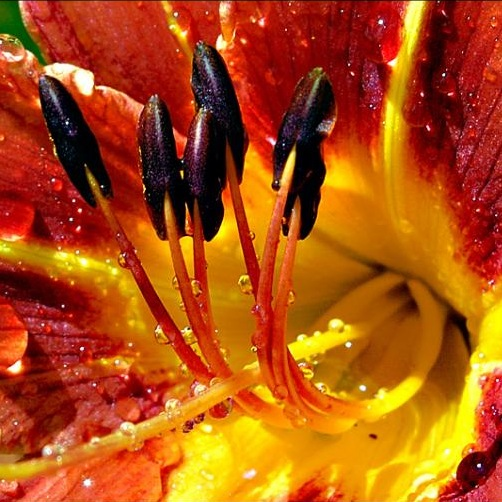
\includegraphics[width=0.3\textwidth]{flowers.png}
	%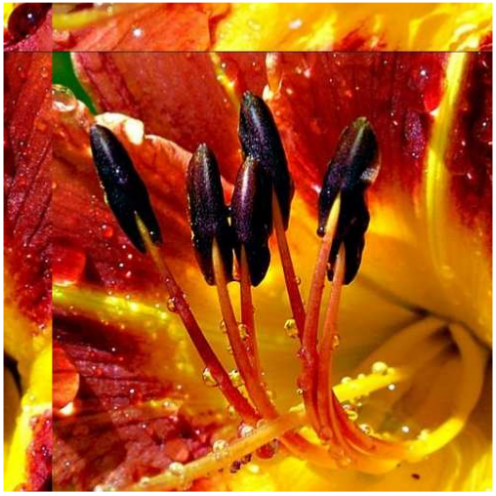
\includegraphics[width=0.3\textwidth]{flowers-translated.png}
  \caption{Image originale, image après rotation}
\end{figure}

\begin{thebibliography}{2}

\bibitem{unser95}
  Unser, Michael, Philippe Thevenaz, and Leonid Yaroslavsky. 
  "Convolution-based interpolation for fast, high-quality rotation of images." 
  IEEE Transactions on Image Processing 4.10 (1995): 1371-1381.
\bibitem{larkin97}  
  Larkin, Kieran G., Michael A. Oldfield, and Hanno Klemm. 
  "Fast Fourier method for the accurate rotation of sampled images." 
  Optics communications 139.1 (1997): 99-106.
\bibitem{paeth86}
	Paeth, Alan W. 
	"A fast algorithm for general raster rotation." 
	Graphics Interface. Vol. 86. 1986.

\end{thebibliography}

\end{document}
